\chapter{Contrôles calendaires et astronomiques}\label{ch:calendrier}

\section{Les dates du jour}

Dans l’ensemble C, \st{nTextesDate} textes contiennent au moins une date convertible en date julienne ; on compte au total \st{nDatesConv} dates converties. Le terme qui précède l’expression calendaire permet d’identifier l’événement daté dans la plupart des cas : déposition (\st{ev_depo}), décès (\st{ev_deces}), naissance (\st{ev_naiss}), achat (\st{ev_achat}) ; \st{ev_indet} dates restent rattachées à un événement indéterminé. Ces nombres comptent des dates, non des textes : un même document peut en contenir plusieurs.

La répartition mensuelle de la première date de chaque texte (figure~\ref{fig:mois}) présente un excédent estival : \st{ete}~\% de ces dates tombent en juillet, août ou septembre. Un test d’ajustement du χ² à une répartition proportionnelle à la longueur des mois donne χ² = \st{chi2} pour onze degrés de liberté (\emph{p} ≈ \st{chi2p}) : l’écart n’atteint pas le seuil conventionnel de 5~\%. L’observation est compatible avec la saisonnalité estivale décrite par Shaw sur un ensemble beaucoup plus large ; elle ne la démontre pas. Elle ne mesure pas non plus la mortalité : l’événement daté est le plus souvent la déposition, et la sélection des textes datés n’a rien d’aléatoire.

\begin{figure}[tbp]\centering
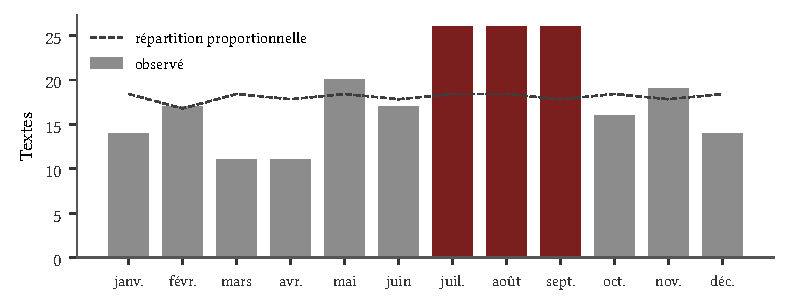
\includegraphics[width=0.9\linewidth]{figures/fig_mois.pdf}
\caption{Mois de la première date convertie de chaque texte de l’ensemble C (n = \st{nMoisTot}) ; trait discontinu : répartition proportionnelle à la longueur des mois.}\label{fig:mois}
\end{figure}

\section{Les jours de la semaine}

Le jour de la semaine est mentionné dix-huit fois dans seize textes. Le tableau~\ref{tab:jours} donne le résultat du contrôle par le calcul du jour julien ; pour les \nnums{55} et 126, la mention se rapporte à la naissance, et le calcul porte sur l’année de la naissance.

% généré par scripts/04_generated.py
\begin{table}[tbp]\centering\footnotesize\setlength{\tabcolsep}{3.5pt}\caption{Contrôle des jours de la semaine (calendrier julien, recalcul ; l’année est celle de l’événement daté : naissance pour les \nnums{55} et 126 première mention).}\label{tab:jours}
\begin{tabular}{@{}r r l l l l l@{}}\toprule N° & Année & Mention & Quantième & Date & Calcul & Résultat\\\midrule
7 & 343 & \lat{die Martis} & \lat{III Nonas Iulias} & 5/7/343 & mardi & concordant \\
55 & 340 & \lat{die Veneris} & \lat{XI Kalendas Iulias} & 21/6/340 & samedi & écart d’un jour \\
118 & 367 & \lat{die Martis} & \lat{—} & — & — & quantième lacunaire \\
122 & 367 & \lat{die Martis} & \lat{Nonis Iuniis} & 5/6/367 & mardi & concordant \\
126 & 350 & \lat{die Saturnis} & \lat{III Idus Augustas} & 11/8/350 & samedi & concordant \\
126 & 368 & \lat{die Saturnis} & \lat{VII Idus Decembres} & 7/12/368 & dimanche & écart d’un jour \\
128 & 368 & \lat{die Martis} & \lat{XV Kalendas Decembres} & 17/11/368 & lundi & écart d’un jour \\
131 & 368 & \lat{die Veneris} & \lat{pridie Nonas Martias} & 6/3/368 & jeudi & écart d’un jour \\
169 & 373 & \lat{die Lunae} & \lat{XV Kalendas Apriles} & 18/3/373 & lundi & concordant \\
275 & 385 & \lat{die Lunae} & \lat{VI Idus Martia} & 10/3/385 & lundi & concordant \\
287 & 386 & \lat{die Solis} & \lat{X Kalendas Septembres} & 23/8/386 & dimanche & concordant \\
349 & 392 & \lat{die Veneris} & \lat{XV Kalendas Octobres} & 17/9/392 & vendredi & concordant \\
381 & 395 & \lat{die Saturni} & \lat{III Idus Maias} & 13/5/395 & dimanche & écart d’un jour \\
381 & 395 & \lat{die Lunae} & \lat{XII Kalendas Iunias} & 21/5/395 & lundi & concordant \\
416 & 397 & \lat{die Veneris} & \lat{tertium Kalendas Iulias} & 29/6/397 & lundi & discordant \\
428 & 398 & \lat{die Saturni} & \lat{XV Kalendas Ianuarias} & 18/12/398 & samedi & concordant \\
428 & 399 & \lat{die Saturni} & \lat{XV Kalendas Ianuarias} & 18/12/399 & dimanche & écart d’un jour \\
431 & 399 & \lat{die Veneris} & \lat{septimum Kalendas Septembres} & 26/8/399 & vendredi & concordant \\
462 & 402 & \lat{die Saturni} & \lat{—} & — & — & quantième lacunaire \\
\bottomrule\end{tabular}\end{table}


Neuf mentions concordent avec la date convertie, et la mention du \nnum{428} concorde si l’on retient 398 plutôt que 399. Dans cinq cas (\nnums{55}, 126 seconde mention, 128, 131 et 381 première mention), l’écart est d’un jour, tantôt dans un sens, tantôt dans l’autre. Ces écarts peuvent tenir à la distinction entre décès et déposition, au rattachement d’un décès nocturne au jour précédent ou suivant, ou à une erreur de gravure ou de lecture ; le corpus ne permet pas de les départager. Au \nnum{416}, le vendredi gravé ne correspond pas au 29 juin 397, qui est un lundi ; l’expression \emph{post ter[tiu]m Kalendas Iulia[s]} est d’interprétation incertaine, et la conversion elle-même doit être tenue pour douteuse. Pour les \nnums{118} et 462, le quantième est perdu.

\section{Deux mentions de l’âge de la lune}

Le \nnum{287} associe un jour de la semaine (\emph{[di]e Sol⸢i⸣s}), un âge de la lune (\emph{[Lu]na XII}) et un signe zodiacal (\emph{[Capricor]nus}) à une date dont le quantième est entièrement restitué par l’éditeur (\emph{[X Kal(endas) Sept(embres)]}). L’année 386 est donnée par la formule consulaire, dont le nom d’Honorius est lu. Le calcul montre que la restitution est compatible avec les indications conservées : le 23 août 386 (julien) est un dimanche ; l’éphéméride donne pour ce jour un âge de la lune compris entre 11,5 jours (à minuit) et 12,5 jours (à 24~h) depuis la nouvelle lune du 11 août, et une longitude écliptique comprise entre 285,6° et 300,6°, dans le signe du Capricorne (270°–300°). Ce n’est pas une confirmation indépendante : si l’éditeur a restitué le quantième à partir de ces mêmes données, le raisonnement serait circulaire. Le fondement de la restitution doit être vérifié dans l’édition.

Le \nnum{349} date la mort de Leoparda du 15\textsuperscript{e} jour avant les calendes d’octobre (17 septembre), un vendredi, \emph{luna XV}. Ce texte ne contient aucun élément consulaire, ni dans l’EDCS ni dans l’EDB : son année (392) provient de la base. Le 17 septembre 392 est bien un vendredi, et l’âge de la lune est ce jour-là compris entre 13,5 et 14,5 jours (nouvelle lune du 3 septembre), ce qui correspond au quatorzième ou au quinzième jour de la lunaison selon le mode de décompte. Le jour de la semaine et l’âge de la lune fournissent ainsi un test de compatibilité avec l’année proposée, sans en démontrer à eux seuls l’unicité.

\section{Naissance, âge et décès}

Trois textes permettent de vérifier la cohérence entre une date de naissance, un âge et une date de décès.

Au \nnum{15}, Cassia, née le 15 juin 316 (consulat de Sabinus et Rufinus) et morte le 15 septembre 346, a vécu « 30 ans et 93 jours » : du 15 juin au 15 septembre on compte 92 jours, soit 93 en décompte inclusif. La durée gravée est donc exactement cohérente avec les deux dates, et le cas confirme que le post-consulat d’Amantius et Albinus désigne 346.

Au \nnum{55}, le calcul conduit de la naissance (21 juin 340) à la déposition (27 septembre 359), conformément au quantième gravé. Le jour de naissance est dit \emph{die Veneris} ; le calcul julien donne un samedi pour le 21 juin 340. L’écart d’un jour est conservé sans correction.

Au \nnum{126}, du 11 août 350 au 7 décembre 368, on compte 18 ans, 3 mois et 26 jours ; le texte donne 19 ans, 3 mois et 26 jours. Les mois et les jours concordent exactement, sans établir indépendamment la validité des deux dates, tandis que l’écart d’une année reste inexpliqué : décompte inclusif des années, erreur de gravure ou de lecture du chiffre \emph{XVIIII}.
